\documentclass{article}
\usepackage{tikz, comment}
\usepackage{pifont}
\usepackage{fontspec, pgfplots}
\usetikzlibrary{arrows, decorations.markings, decorations.pathreplacing}
\begin{comment}
:Title: Not defined yet
:Tags: absolute value rules;properties of equality, equation rules;equivalence properties of equality;set;trichotomy
:Prob: 0.7644;0.6947;0.6235;0.5993;0.5974
:Author: Prof.Hu Ji-shan, HKUST
:Slug: No name yet

Description Here.........
\end{comment}
\begin{document}\centering 

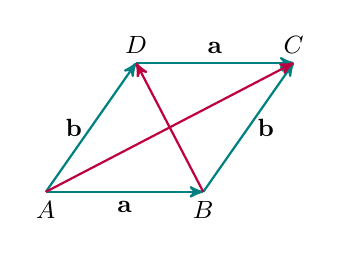
\begin{tikzpicture}[>=latex,xscale=.5*4, yscale=.5*4][font=\sf\small] 

%\draw[xstep=1cm,ystep=1cm,color=gray!80] (-1, -1) grid (4, 5);

\draw[teal, thick, ->, >=stealth'] (0,0)node[black, below]{$A$}
--({1*cos(0)}, {1*sin(0)})node[black, below]{$B$};
\node[below, scale=1] at ({1*cos(0)/2}, {1*sin(0)/2}) {$\bf a$};

\draw[teal, thick, ->, >=stealth'] ({1*cos(0)}, {1*sin(0)})--({1*cos(0)+1*cos(55)}, {1*sin(0)+1*sin(55)})node[black, above]{$C$};
\node[right, scale=1] at ({(1*cos(0) + 1*cos(0)+1*cos(55) )/2}, {(1*sin(0)+1*sin(0)+1*sin(55))/2}) {$\bf b$};

\draw[teal, thick, <-, >=stealth'] 
({1*cos(0)+1*cos(55)}, {1*sin(0)+1*sin(55)})--({1*cos(0)+1*cos(55)+1*cos(-180)}, {1*sin(0)+1*sin(55)+1*sin(-180)})node[black, above]{$D$};
\node[above, scale=1] at ({(1*cos(0)+1*cos(55) + 1*cos(0)+1*cos(55)+1*cos(-180))/2}, {(1*sin(0)+1*sin(55) + 1*sin(0)+1*sin(55)+1*sin(-180))/2}) {$\bf a$};

\draw[teal, thick, <-, >=stealth'] 
({1*cos(0)+1*cos(55)+1*cos(-180)}, {1*sin(0)+1*sin(55)+1*sin(-180)})--(0,0);
\node[left, scale=1] at ({(1*cos(0)+1*cos(55)+1*cos(-180))/2}, {(1*sin(0)+1*sin(55)+1*sin(-180))/2}) {$\bf b$};

\draw[purple, thick, ->, >=stealth'] (0,0)--({1*cos(0)+1*cos(55)}, {1*sin(0)+1*sin(55)});
\draw[purple, thick, ->, >=stealth'] ({1*cos(0)}, {1*sin(0)})--({1*cos(0)+1*cos(55)+1*cos(-180)}, {1*sin(0)+1*sin(55)+1*sin(-180)});

\end{tikzpicture}
\end{document}